\section*{Exercises}

\begin{excersizelist}

\item Sketch the signal
\[
x(t) = e^{-2t} u(t) + e^{t} u(-t)
\]
where $u(t)$ is the step function.  Find the Laplace transform of $x(t)$ and the corresponding region of convergence (ROC).  Sketch the region of convergence on the complex plane.
\begin{solution}
\begin{center}
\begin{tikzpicture}[samples=200]
    %\draw[very thin,color=gray] (-0.1,-1.1) grid (3.9,3.9);
    \draw[->] (-5.1,0) -- (5.1,0) node[above] {$t$};
    \draw[->] (0,-0.3) -- (0,2.3) node[left] {$e^{-2t} u(t) + e^{t} u(-t)$};
    %\draw[color=black] plot[id=x] function{1/x^2} 
    %    node[right] {$f(t) = t^{-2}$};
    \draw[smooth,color=black,domain=-5:0,thick] plot function{2*exp(x)};
    \draw[smooth,color=black,domain=0:5,thick] plot function{2*exp(-2*x)};
    %\draw[color=black] plot[id=exp] function{0.05*exp(x)} 
    %    node[right] {$f(t) = \frac{1}{20} e^t$};
\end{tikzpicture}
\end{center}

The Laplace transform of $e^{-2t}u(t)$ is
\begin{align*}
\calL(e^{-2t}u(t), s) &= \int_{-\infty}^{\infty} e^{-2t}u(t) e^{-st} dt \\
&= \int_{0}^{\infty} e^{-(s+2)t} dt \\
&= -\frac{e^{-(s+2)t}}{s+2} \vert_{0}^\infty \\
&= \frac{1}{s+2}, \qquad \Re(s) > -2
\end{align*}
and the Laplace transform of $e^{t}u(-t)$ is
\begin{align*}
\calL(e^{t}u(-t), s) &= \int_{-\infty}^{0} e^{-(s-1)t} dt \\
&= -\frac{e^{-(s-1)t}}{s-1} \vert_{-\infty}^0 \\
&= -\frac{1}{s-1}, \qquad \Re(s) < 1.
\end{align*}
Thus, the Laplace transform of $e^{-2t} u(t) + e^{t} u(-t)$ is
\[
\calL(e^{-2t} u(t) + e^{t} u(-t), s) = \frac{1}{s+2} - \frac{1}{s-1}, \qquad -2 < \Re(s) < 1
\]
and the region of convergence (ROC) is the subset of the complex plane satisfying $-2 < \Re(s) < 1$.  The unshaded region in the plot below depicts the ROC.

\begin{center}
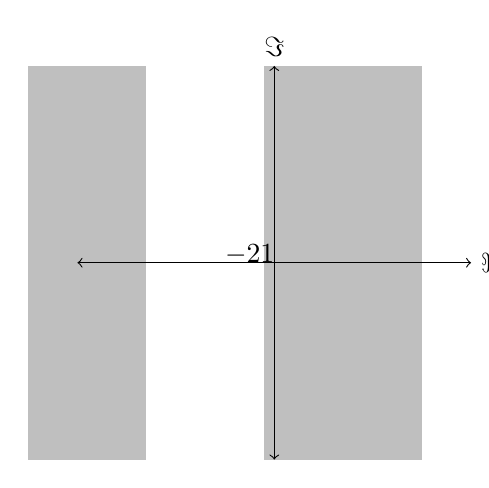
\begin{tikzpicture}
  \path [draw=none,fill=lightgray] (-2.5,-2.5)--(-1,-2.5)--(-1,2.5)--(-2.5,2.5)--cycle;
  \path [draw=none,fill=lightgray] (2.5,2.5)--(0.5,2.5)--(0.5,-2.5)--(2.5,-2.5)--cycle;
  \vtick{-1} node[pos=0.5,below] {$-2$};
  \vtick{0.5} node[pos=0.5,below] {$1$};
  \draw [<->] (-2.5,0) -- (2.5,0) node [right]  {$\Re$};
  \draw [<->] (0,-2.5) -- (0,2.5) node [above] {$\Im$};
\end{tikzpicture}
\end{center}
\end{solution}

\item \label{excer:laplacetransformcommonpolyut} Find the Laplace transform of the signal $t^n u(t)$ where $n\geq 0$ is an integer.
\begin{solution}
We have
\[
\calL\big(t^nu(t)\big) = \int_{-\infty}^{\infty} t^nu(t) e^{-st} dt = \int_{0}^{\infty} t^n e^{-st} dt.
\]
Integration by parts gives the indefinite integral
\[
\int t^n e^{-st} dt = \frac{t^n}{s} e^{-st} + \frac{n}{s} \int t^{n-1} e^{-st} dt.
\]
So, when $\Re(s) > 0$,
\begin{align*}
\calL\big(t^nu(t)\big) &= \lim_{t \to 0}\frac{t^n}{s} e^{-st} - \lim_{t \to \infty}\frac{t^n}{s} e^{-st} + \frac{n}{s} \int_{0}^\infty t^{n-1} e^{-st} dt \\
&= \frac{n}{s} \calL\big(t^{n-1}u(t)\big),
\end{align*}
since both limits converge to zero.  Unravelling the above recursive equation gives
\[
\calL\big(t^nu(t)\big) = \frac{n}{s}\times\frac{n-1}{s}\times\cdots\times\frac{1}{s}\times\calL\big(u(t)\big) = \frac{n!}{s^{n+1}}, \qquad \Re(s) > 0,
\]
since $\calL\big(u(t)\big) = \tfrac{1}{s}$ when $\Re(s) >0$. 
\end{solution}

\item Let $n \geq 0$ be an integer.  Show that the Laplace transform of the signal $- t^n u(-t)$ is the same as the Laplace transform of the signal $t^n u(t)$, but with a different region of convergence.
\begin{solution}
We have
\begin{align*}
\calL\big(-t^nu(-t)\big) &= -\int_{-\infty}^{\infty} t^nu(-t) e^{-st} dt \\
&= \int_{-\infty}^{\infty} (-t)^{n+1} u(t) e^{st} dt \qquad \text{(change variable t = -t)} \\
&= (-1)^{n+1} \int_{-\infty}^{\infty} t^n u(t) e^{st} dt \\
&= (-1)^{n+1} \calL( t^n u(t), -s) \qquad \Re(s) < 0 \\
&= (-1)^{n+1} \frac{n!}{(-s)^{n+1}} \qquad \Re(s) < 0 \\
&= \frac{n!}{s^{n+1}} \qquad \Re(s) < 0.
\end{align*}
\end{solution}

\item \label{exer:finhandroch} Let $H$ be a regular system with impulse response $h$.  Show that the complex exponential signal $e^{st} \in \fin(h)$ if and only if $s \in \roc(h)$.

\item \label{exer:laplacetranstimeshift} Show that equation~\zeqref{eq:transferLaplcetheorem} on page~\zpageref{eq:transferLaplcetheorem} holds when the system $H$ the time shifter $T_\tau$. 
\begin{solution}
Put $y = T_\tau x = x(t- \tau)$.  Taking Laplace transforms
\begin{align*}
\calL y &= \calL T_\tau x \\
&= \int_{-\infty}^{\infty} T_\tau x(t) e^{-st} dt \\
&= \int_{-\infty}^{\infty} x(t - \tau) e^{-st} dt \\
&= \int_{-\infty}^{\infty} x(\kappa) e^{-s(\kappa + \tau)} d\kappa \qquad \text{(ch. vars. $\kappa = t - \tau$)} \\
&= e^{-s\tau}\int_{-\infty}^{\infty} x(\kappa) e^{-s\kappa} d\kappa \\
&= e^{-s\tau} \calL x \qquad s \in \roc(x) \\
&= \lambda T_\tau  \calL x \qquad s \in \roc(x)
\end{align*}
as required.  Observe that the region of convergence of $\calL y$ is the same as that of $\calL x$.
\end{solution}

\item \label{exer:laplacetranstimeshift} Show that equation~\zeqref{eq:transferLaplcetheorem} on page~\zpageref{eq:transferLaplcetheorem} holds when the system $H$ is the differentiator under the added assumption that the limits $\lim_{t\to\infty} x(t) e^{-st}$ and $\lim_{t\to-\infty} x(t) e^{-st}$ both converge to zero when $s \in \roc(x)$. 
\begin{solution}
% We now show the result for the differentiator $D$.  The argument we use is based on that of \citet[page~179]{Rudin_real_and_complex_analysis}.  We have just shown that the Laplace transform of the time shifted $T_{-\tau}(x,t) = x(t + \tau)$ is $e^{\tau s}\calL(x,s)$ with region of convergence $R_x$.  Since the Laplace transform is linear
% \[
% \calL\left( \frac{T_{-\tau}(x) - x}{\tau} \right) =  \frac{e^{\tau s} - 1}{\tau}\calL(x).
% \]
% We now consider what happens to both sides of this equation as $\tau \to 0$.  Application of L'Hopitals rule shows that
% \[
% \lim_{\tau \to 0}\frac{e^{\tau s} - 1}{\tau} = s,
% \]
% and so, the right hand side satisfies
% \[
% \lim_{\tau \to 0} \frac{e^{\tau s} - 1}{\tau}\calL(x) = s \calL(x).
% \]
% On the left hand side we have
% \[
% \lim_{\tau \to 0} \calL\left( \frac{T_{-\tau}(x) - x}{\tau} \right) = \lim_{\tau \to 0} \int_{-\infty}^\infty  \frac{x(t+\tau) - x(t)}{\tau} e^{-st} dt.
% \]
% Observe that
% \[
% \lim_{\tau \to 0} \frac{x(t+\tau) - x(t)}{\tau} = D(x)
% \]
% by definition of the differentiator $D$.  Lebesgue's dominated convergence theorem~\cite[page~26]{Rudin_real_and_complex_analysis} can be used to justify exchanging limits and integration so that
% \begin{align*}
%  \lim_{\tau \to 0} \int_{-\infty}^\infty  \frac{x(t+\tau) - x(t)}{\tau} e^{-st} dt &=  \int_{-\infty}^\infty  \lim_{\tau \to 0} \frac{x(t+\tau) - x(t)}{\tau} e^{-st} dt \\
% &= \int_{-\infty}^\infty D(x,t) e^{-st} dt = \calL\big(D(x)\big).
% \end{align*}
% We now have  $\calL\big(D(x)\big) = s\calL(x) = \lambda(D) \calL(x)$ as required.

Put $y = Dx$.  Taking Laplace transforms
\[
\calL y = \calL D x = \int_{-\infty}^{\infty} Dx(t) e^{-st} dt.
\]
Integrating by parts 
\[
\calL y = \big[ x(t) e^{-st} \big]_{-\infty}^\infty + s\int_{-\infty}^{\infty} x(t) e^{-st} dt = \big[ x(t) e^{-st} \big]_{-\infty}^\infty + s\calL x.
\]
and, by assumption, 
\[
\big[ x(t) e^{-st} \big]_{-\infty}^\infty = \lim_{t\to\infty} x(t) e^{-st}  - \lim_{t\to-\infty} x(t) e^{-st} = 0
\] 
whenever $s$ is in the region of convergence of $x$.  In this case $\calL y = s\calL x$ as required.

The result follows for the $k$th differentiator $D^k$ under the assumption that
\[
\lim_{t\to\infty} D^{c}x(t) e^{-st} = 0 \qquad \text{and} \qquad \lim_{t\to-\infty} D^{c}x(t) e^{-st} = 0
\]
for all $c = 1, 2, \dots, k-1$ because
\[
\calL\big( D^k(x) \big) = \calL\big( D(D^{k-1}(x)) \big) = s \calL\big( D^{k-1}(x) \big)
\]
and unravelling this recursion gives
\[
\calL\big( D^k(y) \big) = \underbrace{s \times s \times \dots \times s}_{\text{$k-1$ times}} \times \calL\big( D(y) \big) = s^k \calL( y ) = \lambda(D^k)\calL(y).
\]
\end{solution}


\item What is the transfer function of the integrator system $I_\infty$ and what is its region of convergence? 
\begin{solution}
We have
\[
I_\infty(e^{st}) = \int_{-\infty}^t e^{s\tau} d\tau = \frac{e^{st}}{s} - \lim_{t\to -\infty}\frac{e^{st}}{s}
\]
and the limit exists only when $\Re{s} > 0$ and in this case it is zero.  So
\[
I_\infty(e^{st}) = \frac{1}{s} e^{st} \qquad \Re{s} > 0
\]
and $\lambda(I_\infty) = \tfrac{1}{s}$.
\end{solution}


\item \label{exer:partialfracfirstorder} By partial fractions, or otherwise, assert that
\[
\frac{as}{s+b} = a - \frac{ab}{s+b}
\]
\begin{solution}
Adding and subtracting $ab$ from the numerator
\[
\frac{as+ab-ab}{s+b} = \frac{a(s+b)-ab}{s+b} = \frac{a(s+b)}{s+b} - \frac{ab}{s+b} = a - \frac{ab}{s+b}
\]
\end{solution}

\item \label{exer:partialfracsecondorder} By partial fractions, or otherwise, assert that
\[
\frac{s + c}{(s+a)(s+b)} = \frac{a-c}{(a-b)(s+a)} + \frac{c-b}{(a-b)(s+b)}
\]
\begin{solution}
Hypothesise the solution
\[
\frac{s + c}{(s+a)(s+b)} = \frac{A}{s+a} + \frac{B}{s+b}.
\]
Multiplying both sides by $(s+a)(s+b)$,
\[
s+c = A(s+b) + B(s+a).
\]
Putting $s = -a$ gives $c-a = A(b-a)$, and pitting $s=-b$ gives $c-b = B(a-b)$, and so,
\[
\frac{s+c}{(s+a)(s+b)} = \frac{a-c}{(a-b)(s+a)} + \frac{c-b}{(a-b)(s+b)}.
\]
\end{solution}

\item \label{exer:partialfracfourthorder} By partial fractions, or otherwise, assert that
\[
\frac{1}{s(s-a)(s-b)(s-b^*)} = \frac{A_0}{s} + \frac{A_1}{s-a} + \frac{A_2}{s-b} + \frac{A_2^*}{s-b^*}
\]
where $a \in \reals$ and $b \in \complex$ and $\Im(b) \neq 0$ and
\[
A_0 = -\frac{1}{a\sabs{b}^2}, \qquad A_1 =  \frac{1}{a\sabs{a - b}^2}, \qquad A_2 = \frac{1}{b(b-a)(b-b^*)}.
\]
You might wish to check your solution using a symbolic programming language (for example Sage, Mathematica, or Maple).
\begin{solution}
The mathemtica command
\begin{verbatim}
Apart[1/s/(s - a)/(s - b)/(s - c), s]
\end{verbatim}
returns the equation
\[
\frac{1}{s(s-a)(s-b)(s-c)} = \frac{A_0}{s} + \frac{A_1}{s-a} + \frac{A_2}{s-b} + \frac{A_3}{s-b^*} -\frac{1}{a b c s}+\frac{1}{}+\frac{1}{}+\frac{1}{ (s-c)}
\]
where
\[
A_0 = -\frac{1}{abc}, \qquad A_1 =  \frac{1}{a (a-b) (a-c)}, 
\]
\[
A_2 = \frac{1}{b (b-a) (b-c)}, \qquad A_3 = \frac{1}{c (c-a) (c-b)}.
\]
Setting $c = b^*$ gives
\[
A_0 = -\frac{1}{a\sabs{b}^2}, \qquad A_1 =  \frac{1}{a\sabs{a - b}^2}, 
\]
\[ 
A_2 = \frac{1}{b(b-a)(b-b^*)}, \qquad A_3 = \frac{1}{b^*(b^*-a)(b^*-b)} = A_2^*
\]
as required.
\end{solution}


\item Let
\[
\calL(y) = \frac{2s + 1}{s^2 + s - 2}
\]
be the Laplace transform of a signal $y$.  By partial fractions, or otherwise, find all possible signals $y$ and their regions of convergence. 
\begin{solution}
Factorise the polynomial on the denominator
\[
\frac{2s + 1}{(s+2)(s-1)}.
\]
Adding and subtracting $s-1$ on the numerator 
\begin{align*}
\frac{2s + 1 + (s-1) - (s-1)}{(s+2)(s-1)} &= \frac{s-1}{(s-1)(s+2)} + \frac{s+2}{(s-1)(s+2)} \\
&= \frac{1}{s+2} + \frac{1}{s-1}.
\end{align*}
There are two time domain signals with Laplace transform $\frac{1}{s+2}$,
\[
e^{-2t} u(t), \; \Re(s) > -2 \qquad \text{and} \qquad -e^{-2t}u(-t), \; \Re(s) < -2,
\] 
and two time domain signals with Laplace transform $-\frac{1}{s-1}$,
 \[
e^{t}u(t), \; \Re(s) > 1 \qquad \text{and} \qquad -e^{t} u(-t), \; \Re(s) < 1.
\] 
There are three possible signals with nonempty regions of convergence
\[
y(t) = e^{-2t} u(t) - e^{t} u(-t) \qquad -2 < \Re(s) < 1,
\]
\[
y(t) = e^{-2t} u(t) + e^{t} u(t) \qquad 1 < \Re(s),
\]
\[
y(t) = - e^{-2t} u(-t) - e^{t} u(-t) \qquad \Re(s) < -2.
\]
\end{solution}

\item \label{excer:timescalelaplace} Let $x$ be a signal with region of convergence $R$.  Show that the time scaled signal $x(\alpha t)$ with $\alpha \neq 0$ satisfies equation~\zeqref{eq:timescalingpropertrylaplacetrans} on page~\zpageref{eq:timescalingpropertrylaplacetrans}.
\begin{solution}
First consider when $\alpha = -1$ so that $x(-t)$ is the reflection of the signal $x$ in time (see Section~\zref{sec:some-import-syst}).  We have 
\begin{align*}
 \calL\big( x(-t), s \big) &=  \int_{-\infty}^{\infty} x(-t)  e^{-s t} dt \\
 &=  -\int_{\infty}^{-\infty} x(\tau)  e^{s\tau} d\tau & \text{(change variable $\tau = -t$)}\\
 &=  \int_{-\infty}^{\infty} x(\tau)  e^{ s \tau} d\tau = \calL(x, -s) \qquad \Re(-s) \in R.
 \end{align*}
 This special case is called the \term{time reversal property}.  Now, when $\alpha > 0$,
 \begin{align*}
 \calL\big( x(\alpha t), s \big) &=  \int_{-\infty}^{\infty} x(\alpha t)  e^{-s t} dt \\
 &=  \frac{1}{\alpha} \int_{\infty}^{\infty} x(\tau)  e^{-s \tau / \alpha}  d\tau & \text{(change variable $\tau = \alpha t$)}\\
 &= \frac{1}{\alpha} \calL(x, s / \alpha) \qquad \Re(s/\alpha) \in R.
 \end{align*}
Combining this with the time reversal property we obtain
 \[
 \calL\big(x(\alpha t),s\big) = \frac{1}{\abs{\alpha}} \calL(x, s/\alpha), \qquad a \neq 0, \Re(s/\alpha) \in R.
 \]
as required.
\end{solution}

% \item \label{exer:thetainfinitelydiff} Plot the signal $\theta(t)$ from~\eqref{eq:thetainfinitediff} and its first 2 derivatives $D(\theta)$ and $D^2(\theta)$. Show that this signal is infinitely differentiable, that is, that it can be differentiated as many times as you like.
% \begin{solution}

% \end{solution}

% \item \label{exer:elevatorgeneralequation} Show that the response of the DC motor to input voltage $v$ from~\eqref{eq:velevatordesigned} satisfies~\eqref{eq:generalequationelevator}.  That is, show that convolution of the impulse response of the motor $h(t) = \tfrac{1}{a} u(t)\big( 1 - e^{-a t/b}\big)$ and the voltage signal $v$ is given by~\eqref{eq:generalequationelevator}.  You may wish to use a symbol programming language (for example Sage, Mathematica, or Maple).
% \begin{solution}
% The following Mathematica commands immediately yield this solution
% \begin{verbatim}
% Theta[t_] := (UnitStep[t] - UnitStep[t - Pi])*Pi*(1-Cos[t]) + 2*Pi*UnitStep[t - Pi];
% v[t_] := 2*Theta'[t] + 3*Theta''[t];
% h[t_, a_, b_] := UnitStep[t]*(1 - Exp[-a/b*t])/a;
% FullSimplify[
% Integrate[
%   h[Tau, a, b]*v[t - Tau], {Tau,-Infinity,Infinity}, 
%   Assumptions -> t Element Reals]]
% \end{verbatim}
% \end{solution}

\item Consider the active electrical circuit from Figure~\zref{elec:activeRC} described by the differential equation from~\zeqref{eq:twoaparrarrelRCactive}.  Derive the transfer function of this system.  Find an explicit system $H$ that maps the input voltage $x$ to the output voltage $y$.  State whether this system is stable and/or regular.
\begin{solution}
The differential equation modelling the circuit is
\[
-\frac{x}{R_1} - C_1 D(x) = \frac{y}{R_2} + C_2 D(y),
\]
and taking Laplace transforms on both sides of this equation
\[
\calL{y} = -\frac{\tfrac{1}{R_1} + C_1s}{\tfrac{1}{R_2} + C_2s} \calL(x) = -\frac{\alpha + \gamma s}{\beta + s}
\]
where $\alpha = \tfrac{1}{R_1C_2}$, $\beta = \tfrac{1}{R_2C_2}$, and $\gamma = \tfrac{C_1}{C_2}$.  The transfer function of the system mapping $x$ to $y$ is correspondingly
\[
\lambda(H) = -\frac{\alpha + \gamma s}{\beta + s} = -\frac{\alpha}{\beta + s} - \frac{\gamma s}{\beta + s}
\]
Applying partial fraction (as in Exercise~\ref{exer:partialfracfirstorder}) to the second term gives
\[
\lambda(H) = -\frac{\alpha + \gamma\beta}{\beta + s} - \gamma
\]
The first term $-\frac{\alpha + \gamma\beta}{\beta + s}$ corresponds with a regular system, say $H_2$, having impulse response
\[
h_2 = -(\alpha + \gamma\beta) u(t) e^{-\beta t}
\]
by using the Laplace transform pair from~\zeqref{eq:laplacetneucommon} with the integer $n=0$.  The term $-\gamma$ correspond with the system $H_1 = \gamma T_0$, i.e, the identity system multiplied by $-\gamma$.  The system $H$ that describes the mapping between input voltage $x$ and output voltage $y$ is thus
\[
H(x) = H_1(x) + H_2(x) = -\gamma x + h_2 * x.
\]
The system is not regular because the $H_1$ is not regular.  The system is stable because $H_1$ is stable and $H_2$ is stable because the impulse response $h_2$ is absolutely integrable since $\beta = \tfrac{1}{R_2C_2} > 0$.  Equivalently the system is not regular because the transfer function does not have more poles than zero, and the system is stable because the transfer function has at least as many poles as zeros (equal in this case), and because all the poles lie strictly in the left half plane. 
\end{solution}

\item \label{exer:massspringdamperrect} Given the mass spring damper system described by~\zeqref{eq:masspringeqseclapltrans}, find the position signal $p$ given that the force signal 
\[
f(t) = \rect\big(t-\tfrac{1}{2}\big) = \begin{cases}
1 & 0 < t \leq 1 \\
0 & \text{otherwise}
\end{cases}
\]
is the rectangular function time shifted by $\tfrac{1}{2}$.  Consider three cases:
\begin{enumerate}
\item $M=1$, $K=\tfrac{\pi^2}{4}$ and $B=\tfrac{\pi}{3}$,
\item $M=1$, $K=\tfrac{\pi^2}{4}$ and $B=\pi$,
\item $M=1$, $K=\tfrac{\pi^2}{4}$ and $B=2\pi$,
\end{enumerate}
Plot the solution in each case, and comment on whether the system is underdamped, overdamped, or critically damped. 
\begin{solution}
Observe that the input force signal can be written as the sum of the step function $u$ and its negated time-shift, that is,
\[
f(t) = u(t) - u(t - 1) = u(t) - T_{1}(u,t)
\]
and so, the response of the linear, time invariant system $H$ modelling the mass spring damper to input force signal $f$ is
\[
H(f) = H\big(u - T_{1}(u)\big) = H(u) - T_{1}\big(H(u)\big),
\]
and so, $H(f,t) = H(u,t) - H(u,t-1)$, where $H(u)$ is the step response of the system.  The step responses are described in Section~\zref{sec:second-order-systems}.  As described in Section~\zref{sec:second-order-systems}, the system is underdamped when $B = \tfrac{\pi}{3}$, critically damped when $B = \pi$ and overdamped when $B = 2\pi$.
\end{solution}

\item Plot the signal $x(t) = \sin(t e^t) u(t)$ and find and plot its derivative $D(x)$.  Show that the region of convergence of $x$ contains those complex numbers $s$ with $\Re(s) > 0$ and that the region of convergence of $D(x)$ contains those with $\Re(s) > 1$.
\begin{solution}
By application of the chain rule the derivative of $\sin(t e^t)$ is $(t+1)e^t \cos(e^t) u(t)$.  These signals are plotted below.
\begin{center}
\begin{tikzpicture}
\begin{scope}[xscale=1.5]
    \draw[->] (-0.5,0) -- (2.8,0) node[above] {$t$};
    \draw[->] (0,-1.3) -- (0,1.3) node[above right] {$\sin(t e^t) u(t)$};
    \draw[thick] (-0.25,0) -- (0,0);
    \draw[smooth,color=black,domain=0:2.5,thick,samples=300] plot function{sin(x*exp(x))};
\end{scope}
\htick{1} node[pos=0.5,left] {$1$};
\htick{-1} node[pos=0.5,left] {$-1$};
\end{tikzpicture}
\end{center}
\begin{center}
\begin{tikzpicture}
\begin{scope}[xscale=1.5,yscale=0.05]
    \draw[->] (-0.5,0) -- (2.8,0) node[above] {$t$};
    \draw[->] (0,-40.3) -- (0,40.3) node[above right] {$(t+1)e^t \cos(t e^t) u(t)$};
    \draw[thick] (-0.25,0) -- (0,0);
    \draw[smooth,color=black,domain=0:2.5,thick,samples=300] plot function{(1+x)*exp(x)*cos(x*exp(x))};
    \draw[smooth,color=black,domain=0:2.45,thick,samples=50,dashed] plot function{(1+x)*exp(x)};
    \draw[smooth,color=black,domain=0:2.45,thick,samples=50,dashed] plot function{-(1+x)*exp(x)};
\end{scope}
\begin{scope}[yscale=0.05]
\htick{30} node[pos=0.5,left] {$30$};
\htick{-30} node[pos=0.5,left] {$-30$};
\end{scope}
\end{tikzpicture}
\end{center}

We have $\abs{x(t)} = \abs{\sin(t e^t) u(t)} < 1$ for all $t \in \reals$ and so
\begin{align*}
\calL\big( x , s\big) &= \int_{-\infty}^\infty \sin(t e^t) u(t) e^{-s t} dt \\
&= \int_{0}^\infty \sin(t e^t) e^{-s t}  dt \\
&\leq = \int_{0}^\infty \abs{\sin(t e^t) e^{-s t}}  dt \\
&\leq \int_{0}^\infty e^{-\Re(s) t}  dt
\end{align*}
which is finite for all $s$ with $\Re(s) > 0$ as required.  For the derivative we have
\begin{align*}
\calL\big( D(x) , s\big) &= \int_{-\infty}^\infty (t+1)e^t \cos(t e^t) u(t) e^{-s t} dt \\
&= \int_{0}^\infty (t+1) \cos(t e^t) e^{-(s-1) t}  dt \\
&\leq \int_{0}^\infty \abs{(t+1) \cos(t e^t) e^{-(s-1) t}}  dt \\
&\leq \int_{0}^\infty (t+1) e^{-(\Re(s)-1) t}  dt
\end{align*}
which is finite for all $s$ with $\Re(s) > 1$ as required.
\end{solution}


\end{excersizelist}

%%% Local Variables: 
%%% mode: latex
%%% TeX-master: "main.tex"
%%% End: 